\documentclass[12pt,a4paper]{article}
\usepackage{graphicx}
\usepackage[utf8]{inputenc}
\usepackage[T5]{fontenc}
\usepackage[top=2.5cm, bottom=2.5cm, left=2.5cm, right=2cm]{geometry}
\usepackage{fancyhdr}
\usepackage{titlesec}
\usepackage{array}
\usepackage{setspace}
\usepackage{tikz}
\usetikzlibrary{positioning,arrows.meta,fit}
\usepackage{hyperref}
\usepackage{tocloft}
\usepackage{float}
\usepackage{makecell}
\usepackage{tabularx}
\usepackage{algpseudocode}
\usepackage{algorithm}
\usepackage{amsmath}
\usepackage{caption}
\usepackage{placeins}
\usepackage{rotating}
\usepackage{longtable}
\usepackage{ragged2e}
\usepackage{enumitem}
\usepackage{subcaption}
\usepackage{indentfirst}
\usepackage{xcolor}
\usepackage{grffile}

\hypersetup{
    colorlinks=true,
    linkcolor=blue,
    urlcolor=blue,
    citecolor=blue
}

\pagenumbering{arabic}
\pagestyle{fancy}
\fancyhf{}
\fancyhead[L]{SmartClock Specification}
\fancyhead[C]{AIoT Project}
\fancyhead[R]{SmartClock}
\renewcommand{\footrulewidth}{0.4pt}
\fancyfoot[L]{University of Science}
\fancyfoot[C]{Faculty of Information Technology}
\fancyfoot[R]{Page \thepage}

\renewcommand{\thealgorithm}{}
\renewcommand{\arraystretch}{1.25}
\setlength{\parindent}{1.2cm}
\setlength{\parskip}{0.2cm}
\newcolumntype{L}{>{\raggedright\arraybackslash}X}
\newcolumntype{P}[1]{>{\raggedright\arraybackslash}p{#1}}

\titleformat{\section}{\Large\bfseries}{\thesection}{1em}{}
\titleformat{\subsection}{\large\bfseries}{\thesubsection}{1em}{}
\titleformat{\subsubsection}{\normalsize\bfseries}{\thesubsubsection}{1em}{}

\begin{document}

\thispagestyle{empty}

\begin{tikzpicture}[remember picture, overlay]
  \draw[blue, line width=3pt] ([xshift=1cm,yshift=-1cm]current page.north west)
    rectangle ([xshift=-1cm,yshift=1cm]current page.south east);
  \draw[blue, line width=3pt] ([xshift=1cm,yshift=-1cm]current page.north west) -- ++(1cm,0);
  \draw[blue, line width=3pt] ([xshift=1cm,yshift=-1cm]current page.north west) -- ++(0,-1cm);
  \draw[blue, line width=3pt] ([xshift=-1cm,yshift=1cm]current page.south east) -- ++(-1cm,0);
  \draw[blue, line width=3pt] ([xshift=-1cm,yshift=1cm]current page.south east) -- ++(0,1cm);
\end{tikzpicture}

\begin{center}
    \vspace{-1cm}
    \textbf{\large VIETNAM NATIONAL UNIVERSITY, HO CHI MINH CITY} \\ [0.3cm]
    \textbf{\Large UNIVERSITY OF SCIENCE} \\ [0.3cm]
    \textit{Faculty of Information Technology} \\
    \vspace{1.5cm}

    \IfFileExists{logo.png}{
      
\includegraphics[width=6cm]{logo.png}
    }{
      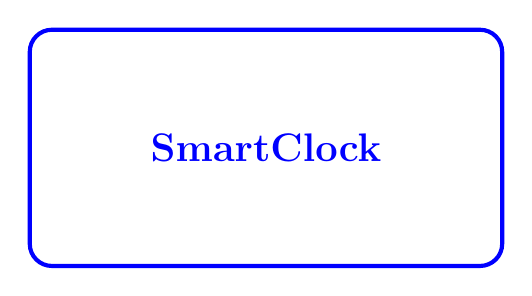
\begin{tikzpicture}
        \draw[blue, line width=1.5pt, rounded corners=8pt] (0,0) rectangle (6,3);
        \node[blue, font=\Large\bfseries] at (3,1.5) {SmartClock};
      \end{tikzpicture}
    } \\
    \vspace{1cm}

    {\LARGE \textbf{SMARTCLOCK SPECIFICATION}} \\[0.5cm]
    {\Large \textbf{AIoT PERSONAL ASSISTANT CLOCK}} \\[0.7cm]
    {\Large Course: Introduction to Smart Device
Programming} \\
    \vspace{1cm}

    \begin{flushleft}
        \textbf{CLASS:} 23CLC02 \\[0.4cm]

        \textbf{PROJECT:} SmartClock - Tập trung hơn, ngủ sâu hơn, sống thông minh hơn. \\[0.5cm]

        \textbf{MEMBER INFORMATION:}
    \end{flushleft}

    \small
    \begin{tabularx}{\textwidth}{|c|P{3cm}|P{1.8cm}|P{2.2cm}|X|}
    \hline
    \textbf{STT} & \textbf{Member} & \textbf{Student ID} & \textbf{Phone Number} & \textbf{Email} \\
    \hline
    1 & Trần Hải Đức & 23127173 & 0916821170 & thduc23@clc.fitus.edu.vn \\
    \hline
    2 & Nguyễn Trọng Tài & 23127008 & 0377425510 & nttai23@clc.fitus.edu.vn  \\
    \hline
    3 & Nguyễn Công Chiến & 23127331 & 0369314655 & ncchien23@clc.fitus.edu.vn \\
    \hline
    4 & Phạm Nguyễn Gia Bảo & 20127119 & 926127333 & pngbao20@clc.fitus.edu.vn  \\
    \hline
    \end{tabularx}
    \normalsize

    \vfill
    \textit{TP.HCM, May 26, 2026.}
\end{center}

\newpage
\tableofcontents
\newpage

\section{Background}

\subsection{Product Overview}

Trong môi trường học tập và làm việc hiện đại, khả năng tập trung đang trở thành một trong những yếu tố quan trọng nhất quyết định hiệu quả công việc và chất lượng cuộc sống. Đặc biệt đối với sinh viên và nhân viên văn phòng, việc duy trì sự tập trung trong thời gian dài ngày càng khó khăn bởi sự xuất hiện liên tục của các yếu tố gây xao nhãng như điện thoại thông minh, mạng xã hội hay thông báo từ các ứng dụng.

Một trong những phương pháp quản lý thời gian phổ biến và hiệu quả hiện nay là phương pháp Pomodoro \cite{pomodoro}. Phương pháp này chia thời gian làm việc thành các khoảng 25 phút tập trung và 5 phút nghỉ ngắn nhằm giúp não bộ duy trì trạng thái làm việc hiệu quả trong thời gian dài. Tuy nhiên, phần lớn các sản phẩm hiện tại chỉ dừng lại ở chức năng đếm thời gian cơ bản, thiếu khả năng cá nhân hóa trải nghiệm người dùng cũng như chưa hỗ trợ các nhu cầu khác liên quan đến học tập và sinh hoạt hằng ngày.

Xuất phát từ ý tưởng đó, nhóm phát triển SmartClock, một thiết bị đồng hồ thông minh không chỉ hỗ trợ tập trung theo phương pháp Pomodoro mà còn được mở rộng với các tính năng hỗ trợ giấc ngủ, giải trí và trang trí không gian làm việc. SmartClock hướng đến trải nghiệm tối giản nhưng hữu ích, giúp người dùng xây dựng thói quen học tập và làm việc hiệu quả hơn.

Sản phẩm được định hướng là một thiết bị nhỏ gọn, thân thiện, dễ sử dụng và phù hợp với nhiều không gian cá nhân như bàn học, bàn làm việc hoặc phòng ngủ.

\begin{center}
\textbf{SmartClock - Tập trung hơn, ngủ sâu hơn, sống thông minh hơn.}
\end{center}

\subsection{Motivation}

Động lực phát triển SmartClock không chỉ đến từ nhu cầu cải thiện hiệu quả học tập và làm việc mà còn xuất phát từ mong muốn tạo ra một sản phẩm công nghệ mang tính thực tiễn cao và có khả năng ứng dụng trong đời sống hằng ngày.

Hiện nay, đa số người dùng sử dụng điện thoại thông minh để quản lý thời gian học tập hoặc đặt nhắc nhở công việc. Tuy nhiên, chính các thiết bị này lại là nguồn gây mất tập trung lớn nhất do sự xuất hiện liên tục của thông báo, mạng xã hội và các nội dung giải trí. Điều này tạo ra nhu cầu về một thiết bị chuyên biệt, tối giản và tập trung vào trải nghiệm hỗ trợ năng suất cá nhân.

Bên cạnh đó, xu hướng phát triển các thiết bị AIoT và Smart Home đang ngày càng phổ biến, mở ra cơ hội cho các sản phẩm thông minh có khả năng tương tác và hỗ trợ người dùng tốt hơn trong cuộc sống hằng ngày. Nhóm phát triển mong muốn tận dụng xu hướng công nghệ này để xây dựng một sản phẩm vừa có giá trị sử dụng thực tế vừa mang tính sáng tạo và hiện đại.

\subsection{Intended Audience}

SmartClock hướng đến các nhóm người dùng có nhu cầu nâng cao khả năng tập trung và tối ưu hiệu quả sinh hoạt cá nhân, bao gồm:

\begin{itemize}
    \item Sinh viên cần cải thiện khả năng tập trung khi học tập và ôn luyện.
    \item Nhân viên văn phòng mong muốn quản lý thời gian làm việc hiệu quả hơn.
    \item Người làm việc tại nhà cần duy trì thói quen làm việc khoa học.
    \item Người muốn cải thiện chất lượng giấc ngủ và xây dựng thời gian sinh hoạt hợp lý.
    \item Người yêu thích các thiết bị công nghệ nhỏ gọn, hiện đại và có tính thẩm mỹ.
\end{itemize}

\subsection{Similar Products and Comparison}

\subsubsection{Smartphone Applications}

Các ứng dụng trên điện thoại như Pomodoro Timer, Forest hoặc Focus To-Do mang lại sự tiện lợi do người dùng có thể dễ dàng cài đặt và sử dụng. Tuy nhiên, điện thoại thông minh cũng chính là nguồn gây xao nhãng lớn nhất bởi thông báo từ mạng xã hội, tin nhắn và nội dung giải trí.

\subsubsection{Smart Watches}

Các thiết bị như Apple Watch hoặc Samsung Galaxy Watch hỗ trợ theo dõi sức khỏe, nhắc nhở công việc và quản lý thời gian khá hiệu quả. Tuy nhiên, đây là các thiết bị đa chức năng với mức giá tương đối cao và vẫn tích hợp nhiều tính năng có khả năng gây phân tâm.

\subsubsection{Traditional Pomodoro Clocks}

Các đồng hồ Pomodoro truyền thống có ưu điểm là đơn giản, dễ sử dụng và giúp hạn chế sự phụ thuộc vào điện thoại. Tuy nhiên, phần lớn các sản phẩm hiện tại chỉ có chức năng hẹn giờ cơ bản và thiếu khả năng mở rộng hoặc cá nhân hóa trải nghiệm người dùng.

\subsubsection{SmartClock Advantages}

\begin{itemize}
    \item Hỗ trợ phương pháp Pomodoro nhằm nâng cao khả năng tập trung.
    \item Hạn chế tối đa các yếu tố gây xao nhãng.
    \item Tích hợp thêm các chức năng hỗ trợ giấc ngủ và giải trí.
    \item Thiết kế nhỏ gọn, phù hợp với không gian học tập và làm việc.
    \item Chi phí tiếp cận hợp lý hơn so với các thiết bị smartwatch cao cấp.
    \item Có khả năng mở rộng thêm các tính năng AIoT trong tương lai.
\end{itemize}

\newpage
\section{Architecture and Hardware}

\subsection{Architecture}

SmartClock được thiết kế theo mô hình AIoT gồm hai thành phần chính: Edge Device và Server. Edge Device là thiết bị SmartClock đặt tại bàn học, bàn làm việc hoặc phòng ngủ của người dùng. Server là hệ thống xử lý, lưu trữ và mở rộng các chức năng thông minh trong tương lai.

Trong mô hình này, Edge Device chịu trách nhiệm tương tác trực tiếp với người dùng thông qua màn hình TFT, năm nút vật lý và các cảm biến. Server đóng vai trò tiếp nhận dữ liệu, lưu lịch sử, hỗ trợ phân tích và cung cấp khả năng mở rộng cho các chức năng AIoT.

\subsubsection{Edge-Server Communication}

SmartClock có thể kết nối với Server thông qua Internet. Vì Edge Device không phải lúc nào cũng được đặt trong môi trường có Wi-Fi cố định, thiết bị có thể truy cập Internet thông qua điện thoại hoặc laptop bằng cách sử dụng hotspot.

Quá trình kết nối có thể chia thành hai pha:

\begin{itemize}
    \item \textbf{Setup / Provisioning Mode:} SmartClock Edge Device phát một Wi-Fi tạm thời, ví dụ \texttt{SmartClock\_Setup}. Người dùng dùng điện thoại hoặc laptop kết nối vào Wi-Fi này để nhập thông tin mạng.
    \item \textbf{Online Mode:} Sau khi nhận cấu hình, SmartClock ngắt mạng setup và kết nối vào Wi-Fi hoặc hotspot của điện thoại/laptop để truy cập Internet và giao tiếp với Server.
\end{itemize}

\begin{center}
\texttt{Phone/Laptop} $\leftrightarrow$ \texttt{SmartClock\_Setup AP}

\texttt{SmartClock Edge Device} $\leftrightarrow$ \texttt{Phone/Laptop Hotspot} $\leftrightarrow$ \texttt{Internet} $\leftrightarrow$ \texttt{SmartClock Server}
\end{center}

\subsubsection{Architecture Diagram}

\begin{figure}[H]
\centering
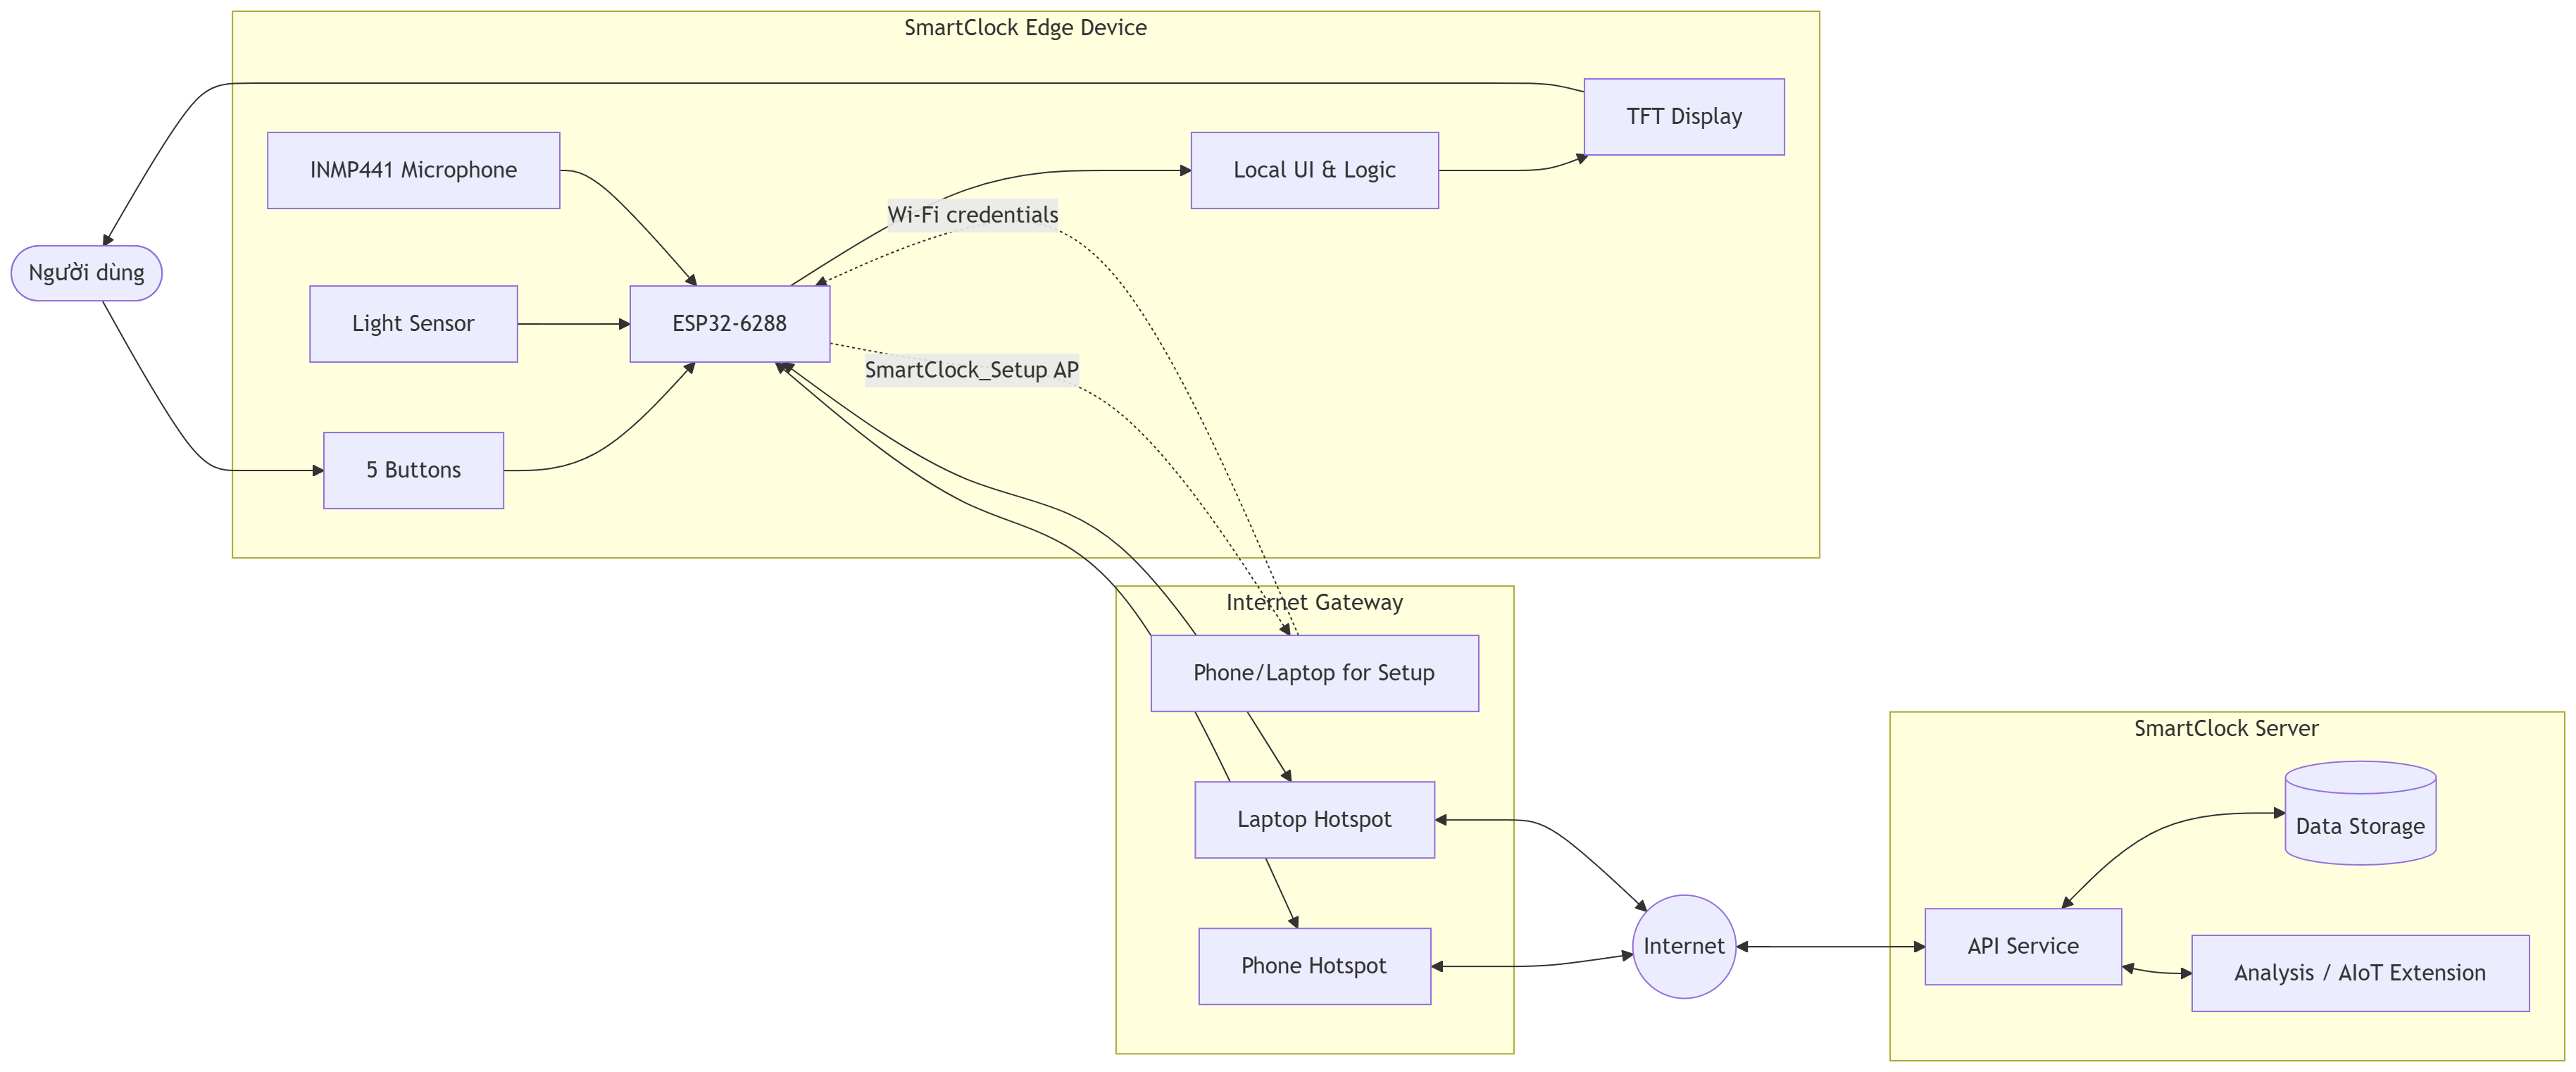
\includegraphics[width=0.95\textwidth]{images/architecture.png}
\caption{SmartClock Edge-Server Architecture}
\label{fig:architecture}
\end{figure}

\subsubsection{Data Flow}

\begin{longtable}{|c|P{12.5cm}|}
\hline
\textbf{Step} & \textbf{Description} \\
\hline
1 & Người dùng thao tác bằng 5 nút vật lý trên SmartClock. \\
\hline
2 & ESP32-6288 xử lý thao tác, cập nhật giao diện TFT và điều khiển chức năng cục bộ. \\
\hline
3 & Cảm biến ánh sáng và INMP441 ghi nhận dữ liệu môi trường khi cần. \\
\hline
4 & Nếu chưa có cấu hình mạng, SmartClock bật Wi-Fi setup để điện thoại hoặc laptop kết nối vào và nhập thông tin Wi-Fi. \\
\hline
5 & SmartClock kết nối Internet thông qua Wi-Fi hotspot từ điện thoại hoặc laptop. \\
\hline
6 & Edge Device gửi dữ liệu hoặc nhận cấu hình từ Server. \\
\hline
7 & Server lưu trữ, phân tích và cung cấp nền tảng mở rộng cho các tính năng AIoT. \\
\hline
\caption{SmartClock Data Flow}
\end{longtable}

\subsubsection{Offline and Online Behavior}

\begin{longtable}{|P{3cm}|P{11.5cm}|}
\hline
\textbf{Mode} & \textbf{Behavior} \\
\hline
Offline & Pomodoro, báo thức, điều hướng menu, Flappy Bird và một số chức năng hiển thị vẫn hoạt động cục bộ. \\
\hline
Online & Thiết bị có thể đồng bộ cấu hình, gửi dữ liệu theo dõi, lưu lịch sử và mở rộng các chức năng phân tích. \\
\hline
\caption{Online and Offline Behavior}
\end{longtable}

\subsection{Hardware}

SmartClock sử dụng các thành phần phần cứng phổ biến, chi phí tương đối thấp và dễ tìm trên thị trường linh kiện điện tử. Bảng dưới đây mô tả các thành phần chính và giá ước lượng.

\begin{longtable}{|P{3cm}|c|P{2.3cm}|P{2cm}|P{4cm}|P{2.3cm}|}
\hline
\textbf{Component} & \textbf{Quantity} & \textbf{Availability} & \textbf{Interface} & \textbf{Purpose} & \textbf{Estimated Price (VND)} \\
\hline
ESP32-S3 DevKitC-1 (N8R8) & 1 & Mua thêm & Wi-Fi, I2S, SPI, I2C & MCU chính, TinyML/Edge AI, đồng bộ Firebase và điều phối các module I2S/SPI. & 150,000 - 220,000 \\
\hline
TFT LCD 2.4'' ILI9341 & 1 & Có sẵn & SPI & Hiển thị toàn bộ UI cho HOME, STUDY, SLEEP và RELAX. & 80,000 - 120,000 \\
\hline
INMP441 MEMS Microphone & 1 & Có sẵn & I2S & Đo âm thanh môi trường, ghi âm Seminar Practice và theo dõi noise khi ngủ. & 40,000 - 55,000 \\
\hline
Cảm biến ánh sáng BH1750 & 1 & Có sẵn & I2C hoặc ADC & Đo light level/quality và kiểm tra phòng tối trước khi ngủ. & 15,000 - 30,000 \\
\hline
Nút nhấn tactile 12x12mm & 5 & Có sẵn 3 nút, mua thêm 2 nút & GPIO Digital & Điều hướng toàn bộ state machine và cấu hình các chức năng. & 5,000/nút; mua thêm khoảng 10,000 \\
\hline
Buzzer passive 5V & 1 & Mua thêm & GPIO PWM & Báo Pomodoro, báo thức Sleep và âm thanh game. & 8,000 \\
\hline
MAX98357A I2S Amp + Loa 0.5W & 1 set & Mua thêm & I2S & Phát nhạc MP3/WAV trong RELAX Music Player. & 35,000 - 60,000 \\
\hline
DS3231 RTC Module (kèm pin) & 1 & Mua thêm & I2C & Kích hoạt báo thức, timestamp Pomodoro và đồng bộ thời gian. & 35,000 \\
\hline
MicroSD Card Module & 1 & Mua thêm & SPI & Lưu file nhạc MP3/WAV cho Music Player. & 25,000 \\
\hline
Pin LiPo 3.7V 1000mAh + TP4056 & 1 & Mua thêm & Power & Nguồn di động tùy chọn cho toàn thiết bị. & 60,000 \\
\hline
\caption{Hardware Components and Estimated Cost}
\label{tab:hardware-cost}
\end{longtable}

\begin{longtable}{|P{5cm}|P{7cm}|}
\hline
\textbf{Cost Type} & \textbf{Estimated Range} \\
\hline
Required additional components & Approximately 418,000 VND \\
\hline
\caption{Estimated Total Cost}
\end{longtable}

Giá trên chỉ mang tính ước lượng cho phiên bản prototype. Chi phí thực tế có thể thay đổi tùy theo nhà cung cấp, chất lượng linh kiện, kích thước màn hình TFT, loại vỏ thiết bị và số lượng sản xuất.

\subsection{Hardware Roles}

\begin{longtable}{|P{3.5cm}|P{11cm}|}
\hline
\textbf{Hardware} & \textbf{Role in SmartClock} \\
\hline
ESP32-6288 & Bộ xử lý trung tâm của Edge Device, chịu trách nhiệm chạy luồng giao diện, đọc nút bấm, đọc cảm biến và kết nối Internet. \\
\hline
TFT Display & Cung cấp giao diện trực quan cho người dùng, bao gồm Home, Study, Sleep và Relax Mode. \\
\hline
5 Buttons & Cho phép người dùng điều khiển thiết bị mà không cần điện thoại, giúp giảm xao nhãng. \\
\hline
Light Sensor & Hỗ trợ ghi nhận điều kiện ánh sáng trong môi trường học tập hoặc nghỉ ngơi. \\
\hline
INMP441 & Hỗ trợ ghi nhận âm thanh môi trường và có thể mở rộng cho chức năng luyện tập thuyết trình. \\
\hline
\caption{Hardware Roles}
\end{longtable}

\subsection{Design Considerations}

\begin{itemize}
    \item \textbf{Tối giản:} Người dùng thao tác bằng 5 nút vật lý, không cần mở điện thoại trong quá trình sử dụng.
    \item \textbf{Chi phí hợp lý:} Các linh kiện được chọn theo tiêu chí phổ biến, dễ mua và phù hợp với prototype.
    \item \textbf{Khả năng mở rộng:} ESP32-6288 có thể kết nối Wi-Fi và giao tiếp với nhiều module cảm biến khác.
    \item \textbf{Tính thực tiễn:} Thiết bị có thể đặt trên bàn học, bàn làm việc hoặc đầu giường.
    \item \textbf{Hoạt động linh hoạt:} SmartClock vẫn dùng được các chức năng cơ bản khi offline và có thể mở rộng khi online.
\end{itemize}

\newpage
\section{Objectives}

\subsection{Overview}

SmartClock được phát triển với mục tiêu trở thành một thiết bị hỗ trợ cá nhân đa chức năng, hướng đến việc nâng cao chất lượng học tập, làm việc và sinh hoạt hằng ngày của người dùng. Thay vì chỉ hoạt động như một chiếc đồng hồ thông thường, SmartClock được định hướng là một thiết bị thông minh có khả năng hỗ trợ tập trung, cải thiện giấc ngủ và tạo trải nghiệm giải trí nhẹ nhàng trong không gian cá nhân.

Các mục tiêu chính của dự án bao gồm:

\begin{itemize}
    \item Hỗ trợ người dùng nâng cao khả năng tập trung và tối ưu hiệu suất làm việc.
    \item Hỗ trợ xây dựng thói quen nghỉ ngơi và cải thiện chất lượng giấc ngủ.
    \item Tạo ra một thiết bị công nghệ nhỏ gọn có khả năng giải trí và trang trí góc học tập hoặc làm việc.
\end{itemize}

\subsection{Overall Use Case Diagram}

\begin{figure}[H]
\centering

\includegraphics[width=0.95\textwidth]{\detokenize{images/UseCase (0).png}}
\caption{Overall SmartClock Use Cases}
\end{figure}

\subsection{Objective 1: Supporting Focus}

Một trong những mục tiêu quan trọng nhất của SmartClock là hỗ trợ người dùng duy trì trạng thái tập trung trong quá trình học tập và làm việc. Hệ thống được thiết kế nhằm giảm thiểu sự phụ thuộc vào điện thoại thông minh và hạn chế các yếu tố gây xao nhãng trong môi trường làm việc.

\begin{figure}[H]
\centering

\includegraphics[width=0.95\textwidth]{\detokenize{images/UseCase (1).png}}
\caption{Objective 1 Use Case Diagram}
\end{figure}

\subsubsection{Use Case 1: Pomodoro Timer}

Pomodoro là một phương pháp quản lý thời gian nổi tiếng nhằm giúp người dùng duy trì sự tập trung trong thời gian dài. Phương pháp này chia thời gian làm việc thành các phiên ngắn, phổ biến nhất là 25 phút tập trung làm việc và 5 phút nghỉ ngơi.

SmartClock tích hợp tính năng Pomodoro Timer nhằm hỗ trợ người dùng xây dựng thói quen học tập và làm việc hiệu quả hơn. Hệ thống cho phép người dùng tùy chỉnh thời gian tập trung và nghỉ ngơi phù hợp với nhu cầu cá nhân.

\textbf{Main Features}
\begin{itemize}
    \item Bắt đầu hoặc tạm dừng phiên Pomodoro.
    \item Tùy chỉnh thời gian tập trung và nghỉ ngơi.
    \item Hiển thị thời gian còn lại theo thời gian thực.
    \item Phát tín hiệu thông báo khi kết thúc phiên làm việc hoặc nghỉ ngơi.
    \item Theo dõi số lượng phiên Pomodoro đã hoàn thành.
\end{itemize}

\begin{longtable}{|P{3.5cm}|P{11cm}|}
\hline
\textbf{Actor} & User \\
\hline
\textbf{Goal} & Tập trung học tập hoặc làm việc hiệu quả hơn. \\
\hline
\textbf{Preconditions} & Thiết bị đã được bật. \\
\hline
\textbf{Main Flow} & Người dùng chọn chế độ Pomodoro, thiết lập thời gian, bắt đầu phiên tập trung, hệ thống đếm thời gian và phát thông báo khi hoàn thành. \\
\hline
\textbf{Expected Result} & Người dùng duy trì được trạng thái tập trung trong thời gian làm việc. \\
\hline
\caption{Pomodoro Timer Use Case}
\end{longtable}

\begin{figure}[H]
\centering

\includegraphics[width=0.88\textwidth]{\detokenize{images/UseCase (2).png}}
\caption{Pomodoro Timer Use Case Diagram}
\end{figure}

\subsubsection{Use Case 2: Seminar Practice}

Seminar Practice cho phép người dùng luyện tập thuyết trình trước thiết bị. Hệ thống hỗ trợ ghi nhận thời gian trình bày và có thể mở rộng thêm khả năng đánh giá tốc độ nói, độ rõ ràng hoặc mức độ tự tin khi thuyết trình.

\textbf{Main Features}
\begin{itemize}
    \item Hỗ trợ đo thời gian thuyết trình.
    \item Ghi nhận thời lượng trình bày.
    \item Hỗ trợ đánh giá cơ bản về bài nói.
    \item Hỗ trợ luyện tập cá nhân.
\end{itemize}

\begin{longtable}{|P{3.5cm}|P{11cm}|}
\hline
\textbf{Actor} & User \\
\hline
\textbf{Goal} & Luyện tập kỹ năng thuyết trình. \\
\hline
\textbf{Preconditions} & Thiết bị hoạt động bình thường. \\
\hline
\textbf{Main Flow} & Người dùng chọn chế độ Seminar Practice, bắt đầu trình bày, hệ thống ghi nhận dữ liệu và hiển thị đánh giá sau khi hoàn thành. \\
\hline
\textbf{Expected Result} & Người dùng cải thiện khả năng trình bày và quản lý thời gian nói. \\
\hline
\caption{Seminar Practice Use Case}
\end{longtable}

\begin{figure}[H]
\centering

\includegraphics[width=0.88\textwidth]{\detokenize{images/UseCase (3).png}}
\caption{Seminar Practice Use Case Diagram}
\end{figure}

\subsection{Objective 2: Supporting Better Sleep}

Ngoài việc hỗ trợ năng suất làm việc, SmartClock còn hướng đến việc cải thiện chất lượng nghỉ ngơi và giấc ngủ của người dùng. Một giấc ngủ tốt giúp nâng cao sức khỏe tinh thần, khả năng tập trung và hiệu suất học tập hoặc làm việc trong ngày hôm sau.

\begin{figure}[H]
\centering

\includegraphics[width=0.95\textwidth]{\detokenize{images/UseCase (4).png}}
\caption{Objective 2 Use Case Diagram}
\end{figure}

\subsubsection{Use Case 1: Sleep Monitoring}

SmartClock hỗ trợ người dùng quan sát thói quen ngủ thông qua việc ghi nhận thời gian đi ngủ, thời gian thức dậy và tổng thời lượng nghỉ ngơi. Dựa trên dữ liệu được ghi nhận, hệ thống hiển thị đánh giá cơ bản để người dùng nhận biết xu hướng giấc ngủ của mình theo từng ngày.

Đây là một tính năng Edge AI của SmartClock. Thiết bị có thể sử dụng một kỹ thuật Machine Learning để xây dựng mô hình đánh giá chất lượng ngủ ngay trên edge device hoặc kết hợp với server khi cần đồng bộ. Input của mô hình bao gồm thời gian ngủ, chất lượng ánh sáng theo thời gian, chất lượng môi trường ngủ theo thời gian, chất lượng âm thanh theo thời gian và các dữ liệu cảm biến liên quan khác. Output của mô hình là điểm số đánh giá chất lượng ngủ, nhận định giấc ngủ có tốt hay không, phân tích nguyên nhân khiến người dùng ngủ không ngon như phòng quá sáng, môi trường quá ồn hoặc thời lượng ngủ chưa phù hợp, đồng thời đưa ra gợi ý cải thiện cho các lần ngủ tiếp theo.

\textbf{Main Features}
\begin{itemize}
    \item Ghi nhận thời gian bắt đầu và kết thúc giấc ngủ.
    \item Tính toán tổng thời lượng ngủ.
    \item Hiển thị đánh giá cơ bản về chất lượng ngủ.
    \item Theo dõi lịch sử giấc ngủ theo ngày.
    \item Gợi ý điều chỉnh thói quen nghỉ ngơi.
\end{itemize}

\begin{longtable}{|P{3.5cm}|P{11cm}|}
\hline
\textbf{Actor} & User \\
\hline
\textbf{Goal} & Theo dõi và cải thiện chất lượng giấc ngủ. \\
\hline
\textbf{Preconditions} & Thiết bị đang hoạt động và người dùng đã chọn chế độ theo dõi giấc ngủ. \\
\hline
\textbf{Main Flow} & Người dùng bật chế độ theo dõi giấc ngủ, hệ thống ghi nhận thời gian ngủ, người dùng kết thúc phiên ngủ và hệ thống hiển thị kết quả. \\
\hline
\textbf{Expected Result} & Người dùng nắm được thời lượng và đánh giá cơ bản về giấc ngủ để điều chỉnh thói quen sinh hoạt. \\
\hline
\caption{Sleep Monitoring Use Case}
\end{longtable}

\begin{figure}[H]
\centering

\includegraphics[width=0.88\textwidth]{\detokenize{images/UseCase (5).png}}
\caption{Sleep Monitoring Use Case Diagram}
\end{figure}

\subsubsection{Use Case 2: Alarm Settings}

SmartClock tích hợp chức năng báo thức tương tự như các thiết bị đồng hồ hoặc điện thoại thông minh hiện nay. Người dùng có thể thiết lập thời gian báo thức nhằm hỗ trợ quản lý lịch sinh hoạt và xây dựng thói quen thức dậy đúng giờ.

\textbf{Main Features}
\begin{itemize}
    \item Thiết lập thời gian báo thức.
    \item Bật hoặc tắt báo thức.
    \item Phát âm thanh thông báo khi đến giờ.
    \item Hỗ trợ nhiều mốc báo thức khác nhau.
\end{itemize}

\begin{longtable}{|P{3.5cm}|P{11cm}|}
\hline
\textbf{Actor} & User \\
\hline
\textbf{Goal} & Thức dậy đúng giờ. \\
\hline
\textbf{Preconditions} & Thiết bị đang hoạt động. \\
\hline
\textbf{Main Flow} & Người dùng thiết lập thời gian báo thức, hệ thống lưu cấu hình, đến thời gian cài đặt, thiết bị phát âm thanh báo thức. \\
\hline
\textbf{Expected Result} & Người dùng nhận được thông báo đúng thời gian mong muốn. \\
\hline
\caption{Alarm Settings Use Case}
\end{longtable}

\begin{figure}[H]
\centering

\includegraphics[width=0.88\textwidth]{\detokenize{images/UseCase (6).png}}
\caption{Alarm Settings Use Case Diagram}
\end{figure}

\subsection{Objective 3: Entertainment and Decoration}

Bên cạnh các chức năng hỗ trợ học tập và sinh hoạt, SmartClock còn được định hướng trở thành một thiết bị có tính giải trí và tính thẩm mỹ, giúp không gian học tập hoặc làm việc trở nên sinh động hơn.

\begin{figure}[H]
\centering

\includegraphics[width=0.95\textwidth]{\detokenize{images/UseCase (7).png}}
\caption{Objective 3 Use Case Diagram}
\end{figure}

\subsubsection{Use Case 1: Flappy Bird}

SmartClock tích hợp một trò chơi mini lấy cảm hứng từ các thiết bị chơi game cầm tay đời cũ. Trò chơi Flappy Bird được xây dựng nhằm tạo ra các khoảng giải trí ngắn sau thời gian học tập hoặc làm việc căng thẳng.

\textbf{Main Features}
\begin{itemize}
    \item Điều khiển nhân vật đơn giản.
    \item Hiển thị điểm số.
    \item Tạo trải nghiệm giải trí nhanh.
    \item Giao diện mang phong cách retro.
\end{itemize}

\begin{longtable}{|P{3.5cm}|P{11cm}|}
\hline
\textbf{Actor} & User \\
\hline
\textbf{Goal} & Giải trí trong thời gian nghỉ ngơi. \\
\hline
\textbf{Preconditions} & Thiết bị đang hoạt động. \\
\hline
\textbf{Main Flow} & Người dùng mở trò chơi, điều khiển nhân vật, hệ thống cập nhật điểm số và kết thúc khi va chạm. \\
\hline
\textbf{Expected Result} & Người dùng có trải nghiệm giải trí nhẹ nhàng. \\
\hline
\caption{Flappy Bird Use Case}
\end{longtable}

\begin{figure}[H]
\centering

\includegraphics[width=0.88\textwidth]{\detokenize{images/UseCase (8).png}}
\caption{Flappy Bird Use Case Diagram}
\end{figure}

\subsubsection{Use Case 2: Music Player}

SmartClock hỗ trợ phát nhạc nhằm tạo không gian thư giãn hoặc hỗ trợ tập trung khi học tập và làm việc. Trong tương lai, tính năng này có thể được mở rộng để hỗ trợ nhiều chế độ âm thanh hoặc kết nối với các nền tảng phát nhạc trực tuyến.

\textbf{Main Features}
\begin{itemize}
    \item Phát nhạc cơ bản.
    \item Điều chỉnh âm lượng.
    \item Chuyển bài hát.
    \item Hỗ trợ âm thanh thư giãn hoặc nhạc tập trung.
\end{itemize}

\begin{longtable}{|P{3.5cm}|P{11cm}|}
\hline
\textbf{Actor} & User \\
\hline
\textbf{Goal} & Nghe nhạc để thư giãn hoặc tập trung. \\
\hline
\textbf{Preconditions} & Thiết bị hoạt động bình thường. \\
\hline
\textbf{Main Flow} & Người dùng chọn chế độ nghe nhạc, chọn bài hát và hệ thống phát âm thanh. \\
\hline
\textbf{Expected Result} & Người dùng có trải nghiệm thư giãn tốt hơn. \\
\hline
\caption{Music Player Use Case}
\end{longtable}

\begin{figure}[H]
\centering

\includegraphics[width=0.88\textwidth]{\detokenize{images/UseCase (9).png}}
\caption{Music Player Use Case Diagram}
\end{figure}

\subsection{Use Case Summary}

\begin{longtable}{|P{3.3cm}|P{3cm}|P{3.3cm}|P{4.2cm}|}
\hline
\textbf{Objective} & \textbf{Use Case} & \textbf{Main Purpose} & \textbf{Expected Result} \\
\hline
Hỗ trợ tập trung & Pomodoro Timer & Quản lý phiên tập trung và nghỉ ngơi & Người dùng duy trì nhịp học tập hoặc làm việc hiệu quả hơn. \\
\hline
Hỗ trợ tập trung & Seminar Practice & Luyện tập thuyết trình và quản lý thời lượng nói & Người dùng cải thiện kỹ năng trình bày. \\
\hline
Hỗ trợ giấc ngủ & Sleep Monitoring & Theo dõi thời lượng ngủ và nhận đánh giá cơ bản & Người dùng hiểu rõ hơn về thói quen nghỉ ngơi. \\
\hline
Hỗ trợ giấc ngủ & Alarm Settings & Thiết lập và quản lý thời gian báo thức & Người dùng thức dậy đúng thời gian mong muốn. \\
\hline
Giải trí và trang trí & Flappy Bird & Giải trí ngắn trong thời gian nghỉ & Người dùng có trải nghiệm thư giãn nhẹ nhàng. \\
\hline
Giải trí và trang trí & Music Player & Phát nhạc thư giãn hoặc nhạc tập trung & Người dùng tạo được không gian phù hợp hơn. \\
\hline
\caption{Use Case Summary}
\end{longtable}

\newpage
\section{Edge AI}

\subsection{Overview}

Từ các mục tiêu đã trình bày ở phần trước, SmartClock không chỉ là một thiết bị hiển thị thời gian hoặc hỗ trợ Pomodoro, mà còn được định hướng trở thành một thiết bị AIoT có khả năng quan sát ngữ cảnh sinh hoạt của người dùng. Trong đó, nhóm chức năng liên quan đến giấc ngủ là phần thể hiện rõ nhất vai trò của Edge AI.

Edge AI trong SmartClock được dùng để xử lý dữ liệu gần người dùng, giảm phụ thuộc hoàn toàn vào Server và cho phép thiết bị đưa ra nhận định cơ bản ngay tại Edge Device. Đối với tính năng Sleep Monitoring, hệ thống có thể thu thập dữ liệu từ cảm biến ánh sáng, microphone, nhiệt độ, môi trường phòng ngủ và gối thông minh FSR để suy luận trạng thái ngủ của người dùng.

Mục tiêu của phần này là mô tả cách SmartClock có thể mở rộng từ chức năng theo dõi thời lượng ngủ đơn giản thành một module phân tích giấc ngủ có khả năng ước lượng trạng thái REM/NREM.

\subsection{Sleep Stage Inference Problem}

Giấc ngủ của con người thường được chia thành hai trạng thái chính:

\begin{itemize}
    \item \textbf{NREM (Non-Rapid Eye Movement):} Giai đoạn ngủ không có chuyển động mắt nhanh, cơ thể thường ổn định và thư giãn hơn, liên quan nhiều đến phục hồi thể chất.
    \item \textbf{REM (Rapid Eye Movement):} Giai đoạn ngủ có chuyển động mắt nhanh, não hoạt động mạnh hơn, thường liên quan đến giấc mơ, xử lý trí nhớ và cảm xúc.
\end{itemize}

Phương pháp chuyên nghiệp để phân tích giấc ngủ là PSG (Polysomnography), sử dụng nhiều tín hiệu sinh lý như EEG, EOG, EMG, ECG và hô hấp. Tuy nhiên, PSG cần thiết bị chuyên dụng, khó sử dụng trong môi trường nhà ở hằng ngày và không phù hợp với mục tiêu prototype nhỏ gọn của SmartClock.

Vì vậy, bài toán của SmartClock được đặt ra là ước lượng trạng thái ngủ REM/NREM của người dùng bằng các tín hiệu thu được từ gối thông minh FSR, âm thanh, nhiệt độ và môi trường phòng ngủ. Hệ thống không nhằm thay thế thiết bị y tế hoặc PSG chuyên nghiệp, mà cung cấp một ước lượng có tính hỗ trợ để người dùng hiểu rõ hơn về thói quen nghỉ ngơi.

\subsection{Input Data}

\begin{longtable}{|P{3.5cm}|P{4.5cm}|P{7cm}|}
\hline
\textbf{Nguồn dữ liệu} & \textbf{Tín hiệu thu thập} & \textbf{Ý nghĩa đối với bài toán} \\
\hline
Gối thông minh FSR & Tư thế ngủ, áp lực đầu/cổ, số lần trở mình & Phát hiện tư thế, mức độ vận động và thay đổi tư thế trong đêm. \\
\hline
Microphone INMP441 & Tiếng ngáy, âm thanh môi trường khi ngủ & Phân tích hiện tượng ngáy, tiếng ồn và biến động âm thanh. \\
\hline
Cảm biến nhiệt độ & Nhiệt độ cơ thể, nhiệt độ phòng & Theo dõi thay đổi thân nhiệt và điều kiện phòng ngủ. \\
\hline
Cảm biến môi trường & CO2, ánh sáng, độ ẩm & Đánh giá chất lượng môi trường ngủ và các yếu tố ảnh hưởng đến giấc ngủ. \\
\hline
Dữ liệu thời gian & Giờ bắt đầu ngủ, giờ thức dậy, tổng thời lượng ngủ & Cung cấp ngữ cảnh theo phiên ngủ và hỗ trợ tính điểm chất lượng ngủ. \\
\hline
\caption{Edge AI Input Data for Sleep Monitoring}
\end{longtable}

Trong phiên bản prototype, SmartClock có thể bắt đầu với các dữ liệu dễ thu thập hơn như ánh sáng, âm thanh và thời lượng ngủ. Các nguồn dữ liệu như FSR, CO2, độ ẩm hoặc nhiệt độ cơ thể có thể được bổ sung ở các phiên bản mở rộng.

\subsection{Expected Output}

Đầu ra của module Edge AI bao gồm:

\begin{itemize}
    \item Nhãn trạng thái ngủ theo từng khoảng thời gian: REM hoặc NREM.
    \item Điểm đánh giá chất lượng giấc ngủ.
    \item Tổng thời lượng ngủ.
    \item Mức độ ổn định của giấc ngủ dựa trên số lần trở mình và biến động âm thanh.
    \item Ghi nhận các yếu tố môi trường bất lợi như phòng quá sáng, quá ồn, CO2 cao hoặc độ ẩm không phù hợp.
    \item Gợi ý cải thiện cho các lần ngủ tiếp theo.
\end{itemize}

\subsection{Edge AI Processing Pipeline}

Quy trình xử lý tổng quát của module Sleep Edge AI:

\begin{center}
\begin{tabular}{c}
\texttt{FSR Pillow / Microphone / Temperature / CO2 / Light / Humidity} \\
$\downarrow$ \\
\texttt{Feature Extraction} \\
$\downarrow$ \\
\texttt{Posture Detection} \\
$\downarrow$ \\
\texttt{Toss and Turn Detection} \\
$\downarrow$ \\
\texttt{Snoring Analysis} \\
$\downarrow$ \\
\texttt{Temperature and Environment Analysis} \\
$\downarrow$ \\
\texttt{Rule-based Sleep Stage Inference} \\
$\downarrow$ \\
\texttt{REM / NREM Prediction} \\
$\downarrow$ \\
\texttt{Heart Rate Comparison / Validation}
\end{tabular}
\end{center}

Trong pipeline này, dữ liệu FSR được dùng để xác định tư thế ngủ và phát hiện thay đổi tư thế; dữ liệu âm thanh được dùng để phát hiện tiếng ngáy, tiếng ồn và các thay đổi bất thường; dữ liệu ánh sáng, nhiệt độ, CO2 và độ ẩm được dùng để đánh giá điều kiện phòng ngủ. Các đặc trưng được trích xuất theo từng cửa sổ thời gian và đưa vào bộ luật suy luận hoặc mô hình Machine Learning nhẹ chạy trên Edge Device.

\subsection{Rule-based Inference Design}

Ở giai đoạn prototype, SmartClock có thể ưu tiên cách tiếp cận rule-based trước khi huấn luyện mô hình phức tạp. Cách này phù hợp với thiết bị nhúng vì dễ triển khai, dễ giải thích và không yêu cầu tài nguyên tính toán lớn.

\begin{longtable}{|P{6cm}|P{8.5cm}|}
\hline
\textbf{Dấu hiệu quan sát} & \textbf{Ý nghĩa suy luận} \\
\hline
Ít thay đổi tư thế, âm thanh ổn định, môi trường tối & Giấc ngủ có xu hướng ổn định hơn, có thể thuộc NREM. \\
\hline
Nhiều biến động âm thanh, nhịp thở hoặc tiếng ngáy thay đổi, cơ thể ít vận động & Có thể là giai đoạn REM hoặc giai đoạn ngủ không ổn định. \\
\hline
Nhiều lần trở mình liên tục & Chất lượng ngủ giảm hoặc người dùng đang ở trạng thái ngủ nông. \\
\hline
Phòng quá sáng hoặc quá ồn & Điều kiện môi trường có thể làm giảm chất lượng giấc ngủ. \\
\hline
CO2 cao, độ ẩm không phù hợp & Môi trường phòng ngủ cần được cải thiện. \\
\hline
\caption{Rule-based Sleep Inference Examples}
\end{longtable}

Trong tương lai, các luật này có thể được thay thế hoặc bổ sung bằng mô hình Machine Learning như Decision Tree, SVM hoặc TinyML model tùy theo tài nguyên của ESP32 và lượng dữ liệu huấn luyện thu thập được.

\subsection{Edge-Server Collaboration}

Edge Device và Server phối hợp theo nguyên tắc:

\begin{itemize}
    \item \textbf{Edge Device} xử lý dữ liệu thời gian thực, đọc cảm biến, trích xuất đặc trưng và đưa ra đánh giá cơ bản ngay tại thiết bị.
    \item \textbf{Server} lưu lịch sử giấc ngủ, tổng hợp dữ liệu theo ngày/tuần, hỗ trợ dashboard và có thể chạy các phân tích nặng hơn.
\end{itemize}

Khi SmartClock offline, thiết bị vẫn có thể ghi nhận phiên ngủ, tính thời lượng ngủ và đưa ra đánh giá cơ bản. Khi online, thiết bị đồng bộ dữ liệu lên Server để người dùng xem lịch sử, biểu đồ hoặc nhận gợi ý cá nhân hóa tốt hơn.

\subsection{Limitations}

\begin{itemize}
    \item Kết quả REM/NREM chỉ là ước lượng hỗ trợ, không phải chẩn đoán y khoa.
    \item Hệ thống không phân tách chi tiết N1, N2, N3 như PSG.
    \item Độ chính xác phụ thuộc vào vị trí cảm biến, chất lượng microphone, nhiễu môi trường và thói quen ngủ của từng người.
    \item Một số cảm biến như FSR, CO2, độ ẩm hoặc nhiệt độ cơ thể có thể chưa có trong phiên bản prototype đầu tiên.
    \item Nếu không có dữ liệu nhịp tim hoặc tín hiệu sinh lý trực tiếp, việc kiểm chứng kết quả REM/NREM sẽ còn hạn chế.
\end{itemize}

\newpage
\section{User Manual}

\subsection{Overview}

Tài liệu này hướng dẫn người dùng thao tác với SmartClock thông qua màn hình TFT và 5 nút vật lý. Các chức năng được tổ chức theo ba nhóm mục tiêu chính: hỗ trợ tập trung, hỗ trợ giấc ngủ, và giải trí/trang trí.

SmartClock sử dụng một nút chuyển chế độ và các nút hành động theo từng màn hình. Người dùng có thể đi qua các chế độ theo vòng lặp:

\begin{center}
\texttt{HOME $\rightarrow$ STUDY $\rightarrow$ SLEEP $\rightarrow$ RELAX $\rightarrow$ HOME}
\end{center}

\subsection{Button Layout}

\begin{longtable}{|P{3cm}|P{11.5cm}|}
\hline
\textbf{Button} & \textbf{Chức năng chung} \\
\hline
Button 1 & Chuyển sang chế độ tiếp theo. \\
\hline
Button 2 & Mở chức năng chính hoặc quay lại menu. \\
\hline
Button 3 & Thực hiện hành động phụ như bắt đầu, tạm dừng hoặc chọn mục. \\
\hline
Button 4 & Tăng giá trị, chuyển bài hoặc mở chức năng bổ sung. \\
\hline
Button 5 & Giảm giá trị, quay bài hoặc mở cấu hình tùy theo màn hình. \\
\hline
\caption{Button Layout}
\end{longtable}

\subsection{Internet Connection Setup}

SmartClock là Edge Device có thể hoạt động cục bộ và có thể kết nối Server khi có Internet. Trong trường hợp không có Wi-Fi cố định, người dùng có thể dùng điện thoại hoặc laptop làm điểm phát Wi-Fi để SmartClock truy cập Internet.

\begin{center}
\texttt{Phone/Laptop} $\leftrightarrow$ \texttt{SmartClock\_Setup AP}

\texttt{SmartClock Edge Device} $\leftrightarrow$ \texttt{Phone/Laptop Hotspot} $\leftrightarrow$ \texttt{Internet} $\leftrightarrow$ \texttt{SmartClock Server}
\end{center}

\subsubsection{Open SmartClock Setup Network}

\begin{enumerate}
    \item Bật SmartClock.
    \item Nếu thiết bị chưa có cấu hình Wi-Fi, SmartClock sẽ bật mạng setup tạm thời, ví dụ \texttt{SmartClock\_Setup}.
    \item Trên điện thoại hoặc laptop, mở danh sách Wi-Fi.
    \item Kết nối vào mạng \texttt{SmartClock\_Setup}.
    \item Mở trang cấu hình của SmartClock nếu thiết bị yêu cầu.
    \item Nhập tên Wi-Fi và mật khẩu mạng sẽ dùng cho SmartClock.
    \item Lưu cấu hình và chờ SmartClock khởi động lại kết nối.
\end{enumerate}

\subsubsection{Connect Through Phone Hotspot}

\begin{enumerate}
    \item Mở phần cài đặt mạng trên điện thoại.
    \item Bật Personal Hotspot hoặc Mobile Hotspot.
    \item Đặt tên Wi-Fi và mật khẩu dễ nhận biết.
    \item Nhập tên hotspot và mật khẩu này vào trang cấu hình SmartClock.
    \item Chờ thiết bị kết nối.
    \item Khi kết nối thành công, SmartClock có thể gửi dữ liệu hoặc nhận cấu hình từ Server.
\end{enumerate}

\subsubsection{Connect Through Laptop Hotspot}

\begin{enumerate}
    \item Kết nối laptop với Internet.
    \item Bật tính năng Mobile Hotspot hoặc Internet Sharing trên laptop.
    \item Kiểm tra tên Wi-Fi và mật khẩu hotspot.
    \item Nhập tên hotspot và mật khẩu này vào trang cấu hình SmartClock.
    \item Chờ trạng thái kết nối thành công.
\end{enumerate}

\begin{longtable}{|P{3cm}|P{11.5cm}|}
\hline
\textbf{Status} & \textbf{Behavior} \\
\hline
Online & SmartClock có thể đồng bộ cấu hình, gửi dữ liệu theo dõi và mở rộng các chức năng phân tích qua Server. \\
\hline
Offline & Pomodoro, báo thức, điều hướng menu, Flappy Bird và một số chức năng cục bộ vẫn có thể hoạt động. \\
\hline
\caption{Online and Offline Usage}
\end{longtable}

\subsection{Home Screen}

Màn hình Home hiển thị tổng quan các nhóm chức năng của SmartClock. Đây là điểm bắt đầu khi thiết bị được bật.

\begin{longtable}{|P{3cm}|P{11.5cm}|}
\hline
\textbf{Button} & \textbf{Action} \\
\hline
Button 1 & Chuyển sang chế độ STUDY. \\
\hline
Button 2-5 & Không sử dụng trên màn hình Home. \\
\hline
\caption{Home Screen Actions}
\end{longtable}

\subsection{Study Mode}

Study Mode hỗ trợ người dùng học tập và làm việc tập trung hơn. Chế độ này gồm Pomodoro Timer và Seminar Practice.

\begin{longtable}{|P{3cm}|P{11.5cm}|}
\hline
\textbf{Button} & \textbf{Action} \\
\hline
Button 1 & Chuyển sang Sleep Mode. \\
\hline
Button 2 & Mở Pomodoro Timer. \\
\hline
Button 3 & Mở Seminar Practice. \\
\hline
\caption{Study Menu Actions}
\end{longtable}

\subsubsection{Pomodoro Timer}

\begin{enumerate}
    \item Vào Study Mode.
    \item Nhấn Button 2 để mở Pomodoro Timer.
    \item Nhấn Button 3 để bắt đầu hoặc tạm dừng bộ đếm.
    \item Nhấn Button 4 để reset bộ đếm về thời gian ban đầu.
    \item Nhấn Button 5 để mở màn hình cấu hình thời gian.
\end{enumerate}

\begin{longtable}{|P{3cm}|P{11.5cm}|}
\hline
\textbf{Button} & \textbf{Pomodoro Configuration Action} \\
\hline
Button 2 & Lưu cấu hình và quay lại Pomodoro Timer. \\
\hline
Button 3 & Chọn trường cần chỉnh: Study Time hoặc Break Time. \\
\hline
Button 4 & Tăng giá trị thêm 1 phút. \\
\hline
Button 5 & Giảm giá trị 1 phút. \\
\hline
\caption{Pomodoro Configuration}
\end{longtable}

\subsubsection{Seminar Practice}

\begin{enumerate}
    \item Vào Study Mode.
    \item Nhấn Button 3 để mở Seminar Practice.
    \item Nhấn Button 3 để bắt đầu ghi nhận phần trình bày.
    \item Nhấn Button 3 lần nữa để kết thúc phần trình bày.
    \item Nhấn Button 4 để xem đánh giá luyện tập.
    \item Nhấn Button 2 để quay lại Study Menu.
\end{enumerate}

\subsection{Sleep Mode}

Sleep Mode hỗ trợ người dùng xây dựng thói quen nghỉ ngơi hợp lý hơn. Chế độ này gồm theo dõi chất lượng ngủ và đặt báo thức.

\begin{longtable}{|P{3cm}|P{11.5cm}|}
\hline
\textbf{Button} & \textbf{Action} \\
\hline
Button 1 & Chuyển sang Relax Mode. \\
\hline
Button 2 & Bắt đầu theo dõi giấc ngủ. \\
\hline
Button 3 & Mở cài đặt báo thức. \\
\hline
Button 4 & Mở cấu hình thời lượng ngủ. \\
\hline
\caption{Sleep Menu Actions}
\end{longtable}

\subsubsection{Sleep Monitoring}

Sleep Monitoring ghi nhận thời gian ngủ và tạo đánh giá cơ bản sau khi người dùng kết thúc phiên theo dõi. Khi module Edge AI được bật, SmartClock có thể kết hợp thêm dữ liệu âm thanh, ánh sáng, nhiệt độ, môi trường phòng ngủ và gối thông minh FSR để ước lượng trạng thái ngủ REM/NREM.

Kết quả REM/NREM chỉ mang tính hỗ trợ theo dõi thói quen nghỉ ngơi, không phải kết luận y khoa. Người dùng nên xem đây là thông tin tham khảo để điều chỉnh môi trường ngủ và lịch sinh hoạt.

\begin{enumerate}
    \item Vào Sleep Mode.
    \item Nhấn Button 2 để bắt đầu theo dõi giấc ngủ.
    \item Để thiết bị hoạt động trong suốt thời gian nghỉ ngơi.
    \item Sau khi thức dậy, nhấn Button 2 để dừng theo dõi.
    \item Xem báo cáo chất lượng ngủ trên màn hình.
    \item Nhấn Button 2 để xác nhận và quay lại Sleep Menu.
\end{enumerate}

\textbf{Sleep Report Information}

Báo cáo sau phiên ngủ có thể bao gồm:

\begin{itemize}
    \item Tổng thời lượng ngủ.
    \item Điểm đánh giá chất lượng giấc ngủ.
    \item Ước lượng tỷ lệ hoặc khoảng thời gian REM/NREM.
    \item Số lần trở mình nếu có dữ liệu từ gối FSR.
    \item Mức độ ngáy hoặc tiếng ồn môi trường nếu có dữ liệu microphone.
    \item Nhận xét về ánh sáng, nhiệt độ, CO2 hoặc độ ẩm phòng ngủ nếu có cảm biến tương ứng.
    \item Gợi ý cải thiện như giảm ánh sáng, giảm tiếng ồn hoặc điều chỉnh thời lượng ngủ.
\end{itemize}

\subsubsection{Alarm Settings}

\begin{enumerate}
    \item Vào Sleep Mode.
    \item Nhấn Button 3 để mở Alarm Settings.
    \item Nhấn Button 3 để bật hoặc tắt báo thức.
    \item Nhấn Button 4 để mở màn hình chỉnh thời lượng ngủ và giờ báo thức.
    \item Nhấn Button 2 để lưu cài đặt và quay lại Sleep Menu.
\end{enumerate}

\begin{longtable}{|P{3cm}|P{11.5cm}|}
\hline
\textbf{Button} & \textbf{Sleep Duration / Alarm Configuration Action} \\
\hline
Button 2 & Lưu cấu hình và quay lại Alarm Settings. \\
\hline
Button 3 & Chọn trường cần chỉnh: Sleep Duration hoặc Alarm Hour. \\
\hline
Button 4 & Tăng giá trị. \\
\hline
Button 5 & Giảm giá trị. \\
\hline
\caption{Sleep and Alarm Configuration}
\end{longtable}

\subsection{Relax Mode}

Relax Mode hỗ trợ người dùng giải trí nhẹ nhàng trong thời gian nghỉ và tăng tính sinh động cho góc học tập hoặc làm việc. Chế độ này gồm Flappy Bird và Music Player.

\begin{longtable}{|P{3cm}|P{11.5cm}|}
\hline
\textbf{Button} & \textbf{Action} \\
\hline
Button 1 & Chuyển về Home Screen. \\
\hline
Button 2 & Mở Flappy Bird. \\
\hline
Button 3 & Mở Music Player. \\
\hline
\caption{Relax Menu Actions}
\end{longtable}

\subsubsection{Flappy Bird}

\begin{enumerate}
    \item Vào Relax Mode.
    \item Nhấn Button 2 để mở Flappy Bird.
    \item Nhấn Button 3 để điều khiển nhân vật nhảy.
    \item Trò chơi kết thúc khi nhân vật va chạm hoặc rơi khỏi vùng chơi.
    \item Nhấn Button 2 để thoát về Relax Menu.
\end{enumerate}

\subsubsection{Music Player}

\begin{enumerate}
    \item Vào Relax Mode.
    \item Nhấn Button 3 để mở Music Player.
    \item Nhấn Button 3 để phát hoặc tạm dừng nhạc.
    \item Nhấn Button 4 để chuyển sang bài tiếp theo.
    \item Nhấn Button 5 để quay lại bài trước.
    \item Nhấn Button 2 để quay lại Relax Menu.
\end{enumerate}

\subsection{Notes}

\begin{itemize}
    \item Trước khi sử dụng, cần đảm bảo SmartClock đã được cấp nguồn và màn hình hiển thị bình thường.
    \item Khi đang cấu hình thời gian, nên kiểm tra kỹ giá trị trước khi nhấn lưu.
    \item Các chức năng đánh giá giấc ngủ, ước lượng REM/NREM và luyện tập seminar trong phiên bản hiện tại mang tính hỗ trợ cơ bản, có thể được mở rộng trong các phiên bản tiếp theo.
    \item Khi dùng Sleep Monitoring, nên đặt SmartClock và các cảm biến liên quan ở vị trí ổn định, hạn chế nguồn tiếng ồn hoặc ánh sáng bất thường để dữ liệu đáng tin cậy hơn.
    \item Kết quả REM/NREM không thay thế thiết bị y tế hoặc phân tích PSG chuyên nghiệp.
    \item Nếu muốn quay lại màn hình chính, tiếp tục nhấn Button 1 để chuyển qua các chế độ theo vòng lặp.
\end{itemize}

\newpage
\section{Conclusion}

\subsection{Project Summary}

SmartClock được xây dựng với định hướng trở thành một thiết bị đồng hồ thông minh nhỏ gọn, dễ sử dụng và phù hợp với không gian học tập, làm việc hoặc nghỉ ngơi cá nhân. Xuất phát từ nhu cầu giảm sự phụ thuộc vào điện thoại thông minh trong quá trình quản lý thời gian, dự án tập trung vào việc tạo ra một thiết bị chuyên biệt có khả năng hỗ trợ người dùng duy trì thói quen sinh hoạt hiệu quả hơn.

Về kiến trúc, SmartClock được thiết kế theo mô hình Edge Device - Server. Thiết bị Edge xử lý tương tác trực tiếp với người dùng, đọc dữ liệu từ cảm biến và hiển thị thông tin trên màn hình TFT. Server đóng vai trò lưu trữ, phân tích và mở rộng các chức năng AIoT trong tương lai. Khi không có Wi-Fi cố định, SmartClock có thể được cấu hình qua mạng setup tạm thời và kết nối Internet thông qua hotspot từ điện thoại hoặc laptop.

Bên cạnh các chức năng như Pomodoro Timer, Seminar Practice, Sleep Monitoring, Alarm Settings, Flappy Bird và Music Player, phần Edge AI giúp SmartClock mở rộng khả năng theo dõi giấc ngủ từ mức ghi nhận thời lượng đơn giản sang hướng phân tích dữ liệu cảm biến, ước lượng REM/NREM và đưa ra gợi ý cải thiện môi trường ngủ.

\subsection{Achieved Objectives}

\subsubsection{Objective 1: Supporting Focus and Productivity}

SmartClock hỗ trợ người dùng làm việc tập trung hơn thông qua Pomodoro Timer. Tính năng này cho phép chia thời gian làm việc thành các phiên tập trung và nghỉ ngơi rõ ràng, giúp người dùng quản lý thời gian hiệu quả mà không cần phụ thuộc vào điện thoại. Seminar Practice mở rộng phạm vi hỗ trợ học tập bằng cách giúp người dùng luyện tập thuyết trình, ghi nhận thời lượng trình bày và xem đánh giá cơ bản sau khi hoàn thành.

\subsubsection{Objective 2: Supporting Better Sleep Habits}

SmartClock hướng đến việc cải thiện chất lượng nghỉ ngơi thông qua chức năng theo dõi giấc ngủ và báo thức. Người dùng có thể bắt đầu phiên theo dõi giấc ngủ, kết thúc phiên khi thức dậy và xem báo cáo đánh giá cơ bản. Khi kết hợp với module Edge AI, hệ thống có thể khai thác dữ liệu âm thanh, ánh sáng, nhiệt độ, môi trường phòng ngủ và gối thông minh FSR để ước lượng trạng thái REM/NREM theo từng khoảng thời gian.

Chức năng báo thức giúp người dùng duy trì thời gian thức dậy ổn định. Khi kết hợp với việc theo dõi thời lượng ngủ, đánh giá điều kiện môi trường và nhận diện các dấu hiệu như tiếng ngáy hoặc số lần trở mình, SmartClock có thể hỗ trợ người dùng hình thành thói quen sinh hoạt điều độ hơn.

\subsubsection{Objective 3: Supporting Relaxation and Workspace Decoration}

Ngoài các chức năng hỗ trợ học tập và nghỉ ngơi, SmartClock còn tích hợp các tính năng giải trí nhẹ như Flappy Bird và Music Player. Các chức năng này giúp thiết bị trở nên sinh động hơn, đồng thời tạo ra khoảng nghỉ ngắn phù hợp sau thời gian học tập hoặc làm việc căng thẳng.

\subsection{User Experience}

SmartClock được thiết kế với luồng sử dụng đơn giản, xoay quanh bốn màn hình chính: Home, Study, Sleep và Relax. Cách tổ chức này giúp người dùng dễ ghi nhớ vị trí của từng chức năng. Việc sử dụng 5 nút vật lý giúp thao tác trở nên trực tiếp và hạn chế sự xao nhãng so với việc sử dụng ứng dụng trên điện thoại.

\subsection{Architecture and Hardware Value}

SmartClock sử dụng các thành phần phần cứng phổ biến như ESP32-6288, TFT Display, 5 nút vật lý, cảm biến ánh sáng và microphone INMP441. Cách lựa chọn linh kiện này giúp sản phẩm có chi phí tiếp cận hợp lý, phù hợp với giai đoạn prototype và vẫn có khả năng mở rộng.

Mô hình Edge-Server giúp SmartClock cân bằng giữa khả năng hoạt động cục bộ và khả năng kết nối thông minh:

\begin{itemize}
    \item Khi offline, thiết bị vẫn có thể sử dụng các chức năng cơ bản như Pomodoro, báo thức, menu, game và một số màn hình hiển thị.
    \item Khi online, thiết bị có thể gửi dữ liệu, nhận cấu hình, lưu lịch sử và mở rộng các chức năng phân tích như dashboard giấc ngủ, tổng hợp REM/NREM hoặc gợi ý cá nhân hóa.
    \item Việc dùng SmartClock làm setup access point tạm thời giúp người dùng cấu hình mạng bằng điện thoại hoặc laptop.
    \item Việc dùng điện thoại hoặc laptop làm hotspot giúp SmartClock linh hoạt hơn trong môi trường học tập, làm việc hoặc thử nghiệm.
\end{itemize}

\subsection{Limitations}

\begin{itemize}
    \item Các chức năng đánh giá giấc ngủ, ước lượng REM/NREM và luyện tập seminar hiện mới dừng ở mức hỗ trợ cơ bản.
    \item Kết quả REM/NREM chỉ là ước lượng dựa trên tín hiệu gián tiếp, không thay thế PSG hoặc chẩn đoán y khoa.
    \item Một số nguồn dữ liệu như gối thông minh FSR, CO2, độ ẩm, nhiệt độ cơ thể hoặc nhịp tim có thể chưa được triển khai đầy đủ trong phiên bản prototype đầu tiên.
    \item Music Player và Flappy Bird chủ yếu phục vụ trải nghiệm mô phỏng hoặc giải trí nhẹ, chưa phải hệ thống giải trí hoàn chỉnh.
    \item Việc kết nối Internet thông qua hotspot phụ thuộc vào chất lượng mạng của điện thoại hoặc laptop.
    \item Cơ chế setup Wi-Fi cần được thiết kế cẩn thận để người dùng nhập thông tin mạng dễ dàng và an toàn.
    \item Chi phí phần cứng hiện mới là ước lượng cho prototype, có thể thay đổi theo thị trường linh kiện.
    \item Chưa có phần đánh giá thực nghiệm với người dùng thực tế để đo mức độ cải thiện tập trung hoặc chất lượng sinh hoạt.
\end{itemize}

\subsection{Future Development}

\begin{itemize}
    \item Hoàn thiện thiết kế mạch, vỏ thiết bị và bố trí linh kiện cho phiên bản prototype ổn định hơn.
    \item Cải thiện thuật toán đánh giá giấc ngủ dựa trên nhiều dữ liệu hơn như ánh sáng, âm thanh, nhiệt độ, CO2, độ ẩm, FSR pillow hoặc thói quen sử dụng.
    \item Mở rộng module Edge AI để phân tích REM/NREM theo từng cửa sổ thời gian và đồng bộ kết quả lên dashboard.
    \item Mở rộng Seminar Practice với khả năng phân tích tốc độ nói, độ rõ ràng, ngữ điệu và mức độ tự tin.
    \item Bổ sung khả năng lưu lịch sử Pomodoro, lịch sử giấc ngủ và kết quả luyện tập.
    \item Cá nhân hóa giao diện và cấu hình theo từng người dùng.
    \item Kết nối với các nền tảng AIoT hoặc Smart Home để tăng khả năng tự động hóa.
    \item Tối ưu cơ chế kết nối Internet, cấu hình Wi-Fi và đồng bộ Edge-Server.
\end{itemize}

\subsection{Final Conclusion}

SmartClock là một dự án có tính thực tiễn cao, xuất phát từ nhu cầu rất phổ biến trong đời sống hiện đại: duy trì sự tập trung, quản lý thời gian, cải thiện giấc ngủ và tạo không gian cá nhân cân bằng hơn. So với các ứng dụng điện thoại hoặc thiết bị đa chức năng dễ gây xao nhãng, SmartClock hướng đến trải nghiệm tối giản, trực tiếp và tập trung vào những nhu cầu thiết yếu.

Với kiến trúc Edge-Server, khả năng cấu hình mạng qua setup access point, kết nối Internet linh hoạt qua điện thoại hoặc laptop, cùng bộ phần cứng prototype có chi phí hợp lý, SmartClock có nền tảng rõ ràng để tiếp tục phát triển thành một sản phẩm AIoT hoàn chỉnh hơn.

\begin{center}
\textbf{SmartClock - Tập trung hơn, ngủ sâu hơn, sống thông minh hơn.}
\end{center}

\newpage
\section{Appendix and Reference}

\subsection{Appendix}

\subsubsection{Key Terms}

\begin{longtable}{|P{3.2cm}|P{11.2cm}|}
\hline
\textbf{Term} & \textbf{Description} \\
\hline
SmartClock & Thiết bị đồng hồ thông minh hỗ trợ tập trung, giấc ngủ và giải trí cá nhân. \\
\hline
Edge Device & Thiết bị xử lý gần người dùng, trực tiếp đọc cảm biến, hiển thị giao diện và nhận thao tác nút bấm. \\
\hline
Server & Thành phần xử lý, lưu trữ và mở rộng các chức năng phân tích hoặc AIoT. \\
\hline
Hotspot & Điểm phát Wi-Fi từ điện thoại hoặc laptop để SmartClock truy cập Internet. \\
\hline
Setup AP & Mạng Wi-Fi tạm thời do SmartClock phát ra để điện thoại hoặc laptop kết nối vào và cấu hình Internet. \\
\hline
Pomodoro & Phương pháp quản lý thời gian bằng cách chia phiên làm việc và nghỉ ngơi. \\
\hline
TFT Display & Màn hình màu dùng để hiển thị giao diện thiết bị. \\
\hline
INMP441 & Microphone digital giao tiếp I2S, dùng để ghi nhận âm thanh. \\
\hline
\caption{Key Terms}
\end{longtable}

\subsection{Screen Flow Summary}

\begin{center}
\texttt{HOME $\rightarrow$ STUDY $\rightarrow$ SLEEP $\rightarrow$ RELAX $\rightarrow$ HOME}
\end{center}

\begin{longtable}{|P{3cm}|P{11.5cm}|}
\hline
\textbf{Mode} & \textbf{Main Use Cases} \\
\hline
HOME & Hiển thị tổng quan và chuyển chế độ. \\
\hline
STUDY & Pomodoro Timer, Seminar Practice. \\
\hline
SLEEP & Sleep Monitoring, Alarm Settings. \\
\hline
RELAX & Flappy Bird, Music Player. \\
\hline
\caption{Screen Flow Summary}
\end{longtable}

\subsection{Hardware Reference Table}

\begin{longtable}{|P{3.5cm}|P{4.5cm}|P{6.2cm}|}
\hline
\textbf{Component} & \textbf{Role} & \textbf{Notes} \\
\hline
ESP32-6288 & Main controller and Wi-Fi connection & Điều khiển giao diện, đọc nút bấm, đọc cảm biến và kết nối Internet. \\
\hline
TFT Display & User interface & Hiển thị menu, timer, báo cáo và trò chơi. \\
\hline
5 Buttons & User input & Điều hướng các chế độ và chức năng. \\
\hline
Light Sensor & Environment sensing & Ghi nhận ánh sáng môi trường. \\
\hline
INMP441 & Audio sensing & Ghi nhận âm thanh môi trường hoặc bài luyện tập. \\
\hline
\caption{Hardware Reference Table}
\end{longtable}

\subsection{Internet Connection Reference}

SmartClock có thể kết nối Internet theo mô hình:

\begin{center}
\texttt{Phone/Laptop} $\leftrightarrow$ \texttt{SmartClock\_Setup AP}

\texttt{SmartClock Edge Device} $\leftrightarrow$ \texttt{Phone/Laptop Hotspot} $\leftrightarrow$ \texttt{Internet} $\leftrightarrow$ \texttt{SmartClock Server}
\end{center}

Khi dùng hotspot, người dùng cần đảm bảo:

\begin{itemize}
    \item Điện thoại hoặc laptop đã bật chia sẻ Internet.
    \item Nếu SmartClock chưa có cấu hình mạng, người dùng kết nối điện thoại hoặc laptop vào \texttt{SmartClock\_Setup} trước.
    \item SmartClock được cấu hình đúng tên Wi-Fi và mật khẩu.
    \item Thiết bị phát hotspot ở đủ gần SmartClock.
    \item Kết nối Internet ổn định nếu cần đồng bộ hoặc phân tích dữ liệu.
\end{itemize}

\begin{thebibliography}{9}
\bibitem{pomodoro}
Pomodoro Technique, Wikipedia. \url{https://en.wikipedia.org/wiki/Pomodoro_Technique}

\bibitem{esp32}
ESP32 Series, Espressif Systems. \url{https://www.espressif.com/en/products/socs/esp32}

\bibitem{inmp441}
INMP441 MEMS Microphone Module, InvenSense / TDK product information. \url{https://invensense.tdk.com/products/digital/inmp441/}

\bibitem{tft}
TFT LCD, Wikipedia. \url{https://en.wikipedia.org/wiki/Thin-film-transistor_liquid-crystal_display}

\bibitem{windows-hotspot}
Mobile hotspot overview, Microsoft Support. \url{https://support.microsoft.com/windows/use-your-windows-pc-as-a-mobile-hotspot-c89b0fad-72d5-41e8-f7ea-406ad9036b85}

\bibitem{android-hotspot}
Android tethering and hotspot help, Google Android Help. \url{https://support.google.com/android/answer/9059108}

\bibitem{nshop-inmp441}
Cảm biến âm thanh INMP441 MEMS I2S, Nshop. \url{https://nshopvn.com/product/cam-bien-am-thanh-inmp441-mems-i2s-micro-da-huong/}

\bibitem{nshop-light}
Cảm biến cường độ ánh sáng quang trở, Nshop. \url{https://nshopvn.com/product/cam-bien-cuong-do-anh-sang-quang-tro/}

\bibitem{linhkienviet-light}
Cảm biến ánh sáng, Linh Kiện Việt. \url{https://linhkienviet.vn/ca-m-bie-n-anh-sang}
\end{thebibliography}

\end{document}

